\chapter{Апробация курса лабораторных работ}

В качестве тестирования курса, было прорешено по одному варианту для каждой лабораторной работы опираясь на представленный код. Отчеты были сохранены в формате notebook, с выходами (графики, ошибки по эпохам и прочее) и выводами.

\section{Лабораторная работа 1}

Был написан классификатор на наборе данных FASHION-mnist.

Архитектура сети аналогична представленной в учебнике из предыдущего раздела. Количество эпох обучения - 5000, что составило примерно 8 минут, на пк без графического процессора. Итоговая точность классификации: 90 процентов.

\begin{figure}[htbp]
\centering
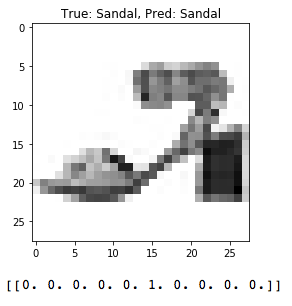
\includegraphics[width=0.7\textwidth]{fig/san}
\caption{Матрица с предсказаниями}%
\label{fig:san}
\end{figure}

В отчете представлены графики выходов со сверточных слоев и значения фильтров (веса).

\begin{figure}[htbp]
\centering
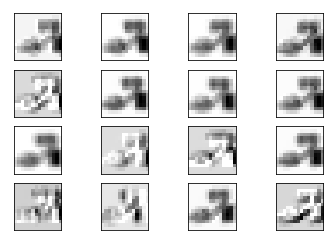
\includegraphics[width=0.7\textwidth]{fig/outsan}
\caption{Выход с первого сверточного слоя}%
\label{fig:san}
\end{figure}

\begin{figure}[htbp]
\centering
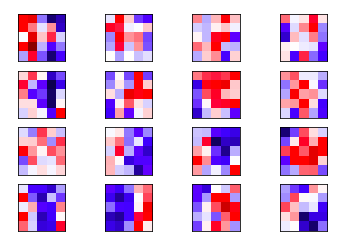
\includegraphics[width=0.7\textwidth]{fig/weig}
\caption{Значения весов (красные - положительные, синие - отрицательные значения)}%
\label{fig:weig}
\end{figure}

\section{Лабораторная работа 2}
Для тестирования второй лабораторной работы, был создан набор данных: собраны и промаркированы изображения, конвертированы метки в формат TFrecord; переобучена модель ssd mobilenet v1 coco на более чем 1000 эпохах, что составило, примерно, 6 часов.

В отчете приведены графики ошибок классификации, локализации и общая ошибка обучения с помощью инструмента визуализации TensorBoard.

\begin{figure}[htbp]
\centering
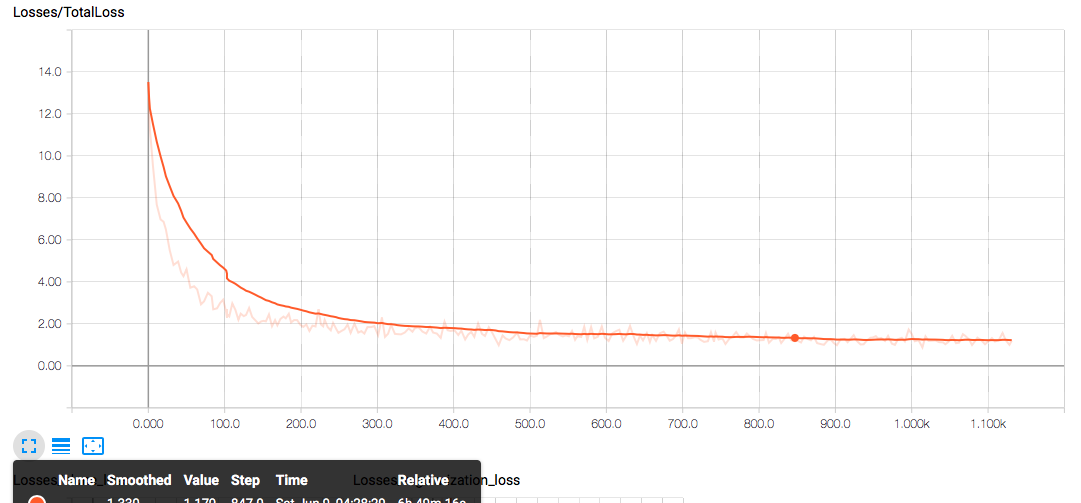
\includegraphics[width=0.7\textwidth]{fig/img3}
\caption{График ошибки обучения}%
\label{fig:san}
\end{figure}

Общая ошибка составила значение около единицы.

\begin{figure}[htbp]
\centering
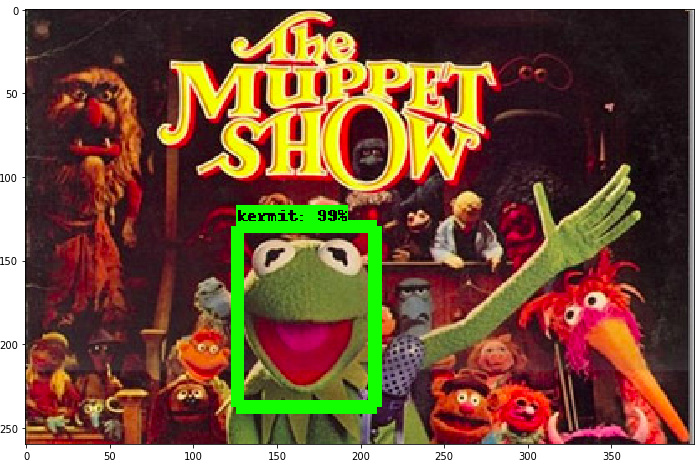
\includegraphics[width=0.7\textwidth]{fig/kermit}
\caption{Результат обучения}
\label{fig:kermit}
\end{figure}

В итоге, получили модель, которая может распознавать и детектировать лягушку на изображениях.

\section{Лабораторная работа 3}
Аналогично первой лабораторной, был решен первый вариант из представленных.


Набор данных содержит информацию о температуре за период времени с 1 января 2010 до 31 декабря 2014 года. Также был разделен набор данных на тестовый и тренировочный в отношении 90 к 10.

\begin{figure}[htbp]
\centering
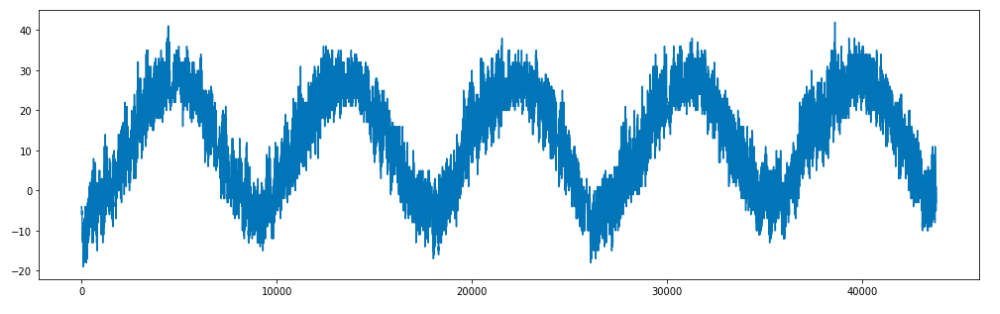
\includegraphics[width=0.7\textwidth]{fig/poll}
\caption{Исходный временной ряд}
\label{fig:poll}
\end{figure}

Для обучения использовали сеть с 1 входом, 1 скрытым слоем, с 8 нейронами и выходным слоем. Обучение было произведено на 200 эпохах и заняло около 15 минут.

\begin{figure}[htbp]
\centering
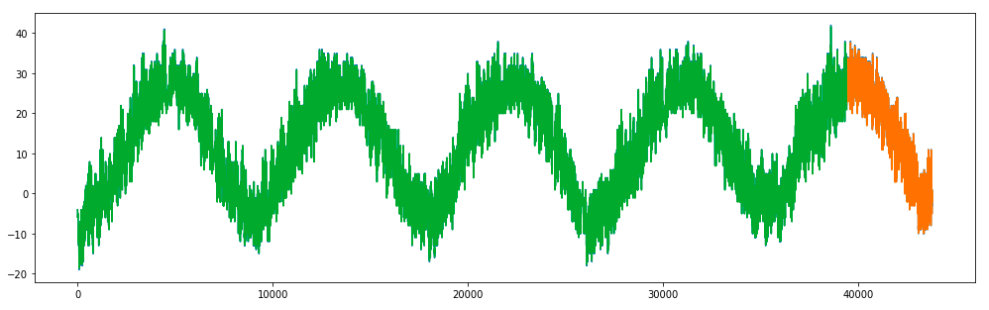
\includegraphics[width=0.7\textwidth]{fig/poll2}
\caption{Результат предсказания (изображено желтым цветом)}
\label{fig:poll}
\end{figure}

Среднеквадратичная ошибка на тренировочном наборе составила - 1.5, на тестовом - 1.48 единиц. Это хороший результат, благодаря тому, что на исходной выборке явно прослеживался периодичный тренд.